\chapter{Imperical results}

\startcontents[chapters]
\printmyminitoc{
}

To do the evaluation, I created similarity matrices to see if topics between clusters were well-separated. The more light color the matrices, the more clusters are being well separated. The score is created by the tf-idf score and we calculate using the Euclidean distance.


\section{MiniLMv2 representation}

The results are very promising. The list of the words after this technique is the theme that right now agents label by hand. We also see that there are topics that are close to each other by the list of the tf-idf most significant words. For example:

\begin{itemize}
    \item euros, facture, mobile, payer, forfait, paye |  about invoices
    \item euros, facture, mois, factures, juillet, pour |  about invoices
    \item maroc, espagne, france, pars, algrie, utilise |  about roaming
    \item sim, code, carte, pin, bloqu, cartes, tlphone | problem with sim card
    \item internet, wifi, rseau, connexion, internet | problem with internet connection
\end{itemize}

However, we could also see that HDBSCAN and PCA are not well put together. The list of words in this case only contains really common words that could appear in any document.

\begin{figure}[H]
    \centering
    \begin{subfigure}{0.45\textwidth}
        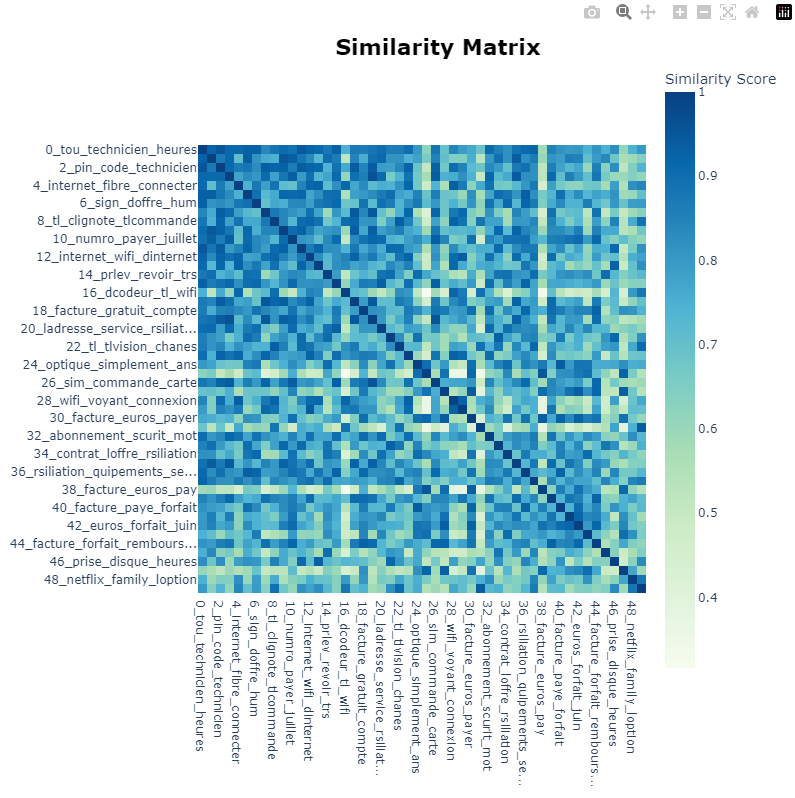
\includegraphics[width=\linewidth]{images/results/mini/kmeans_umap.png}
        \caption{Kmeans - UMAP}
    \end{subfigure}
    \begin{subfigure}{0.45\textwidth}
        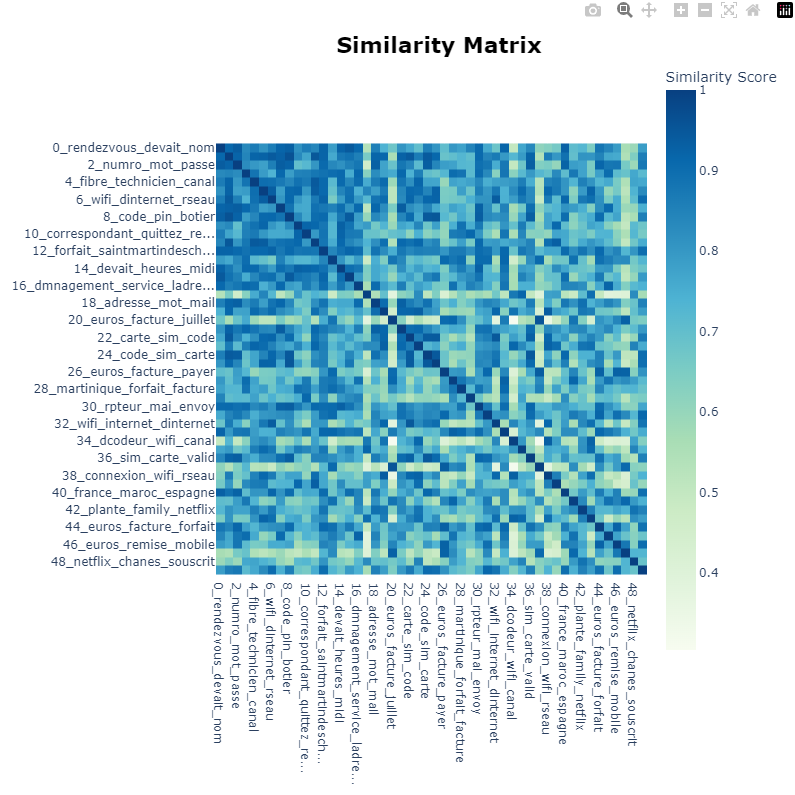
\includegraphics[width=\linewidth]{images/results/mini/kmeans_pca.png}
        \caption{Kmeans - PCA}
    \end{subfigure}
    \caption{Result - miniLMv2}
    \label{fig:result_mini_2}
\end{figure}


\begin{figure}[H]
    \centering
    \begin{subfigure}{0.45\textwidth}
        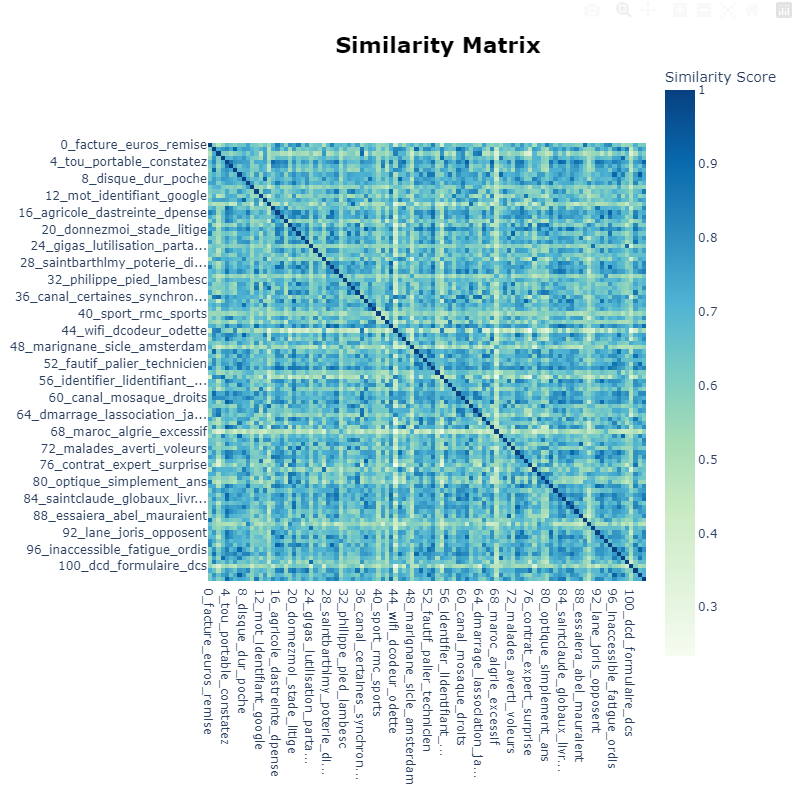
\includegraphics[width=\linewidth]{images/results/mini/hdbscan-umap.png}
        \caption{HDBSCAN - UMAP}
    \end{subfigure}
    \begin{subfigure}{0.45\textwidth}
        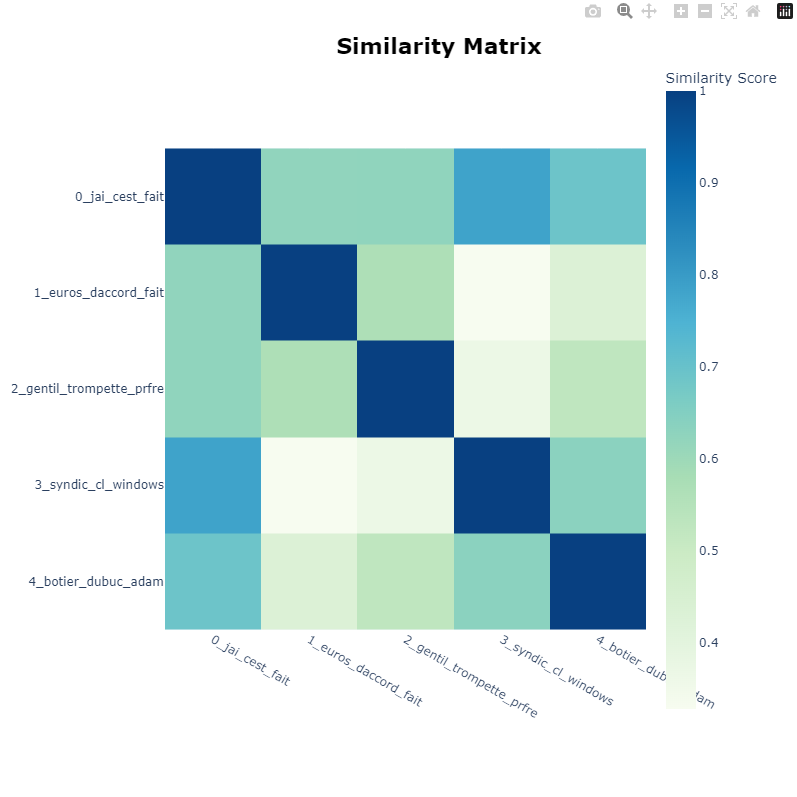
\includegraphics[width=\linewidth]{images/results/mini/hdbscan-pca.png}
        \caption{HDBSCAN - PCA}
    \end{subfigure}
    \begin{subfigure}{0.45\textwidth}
        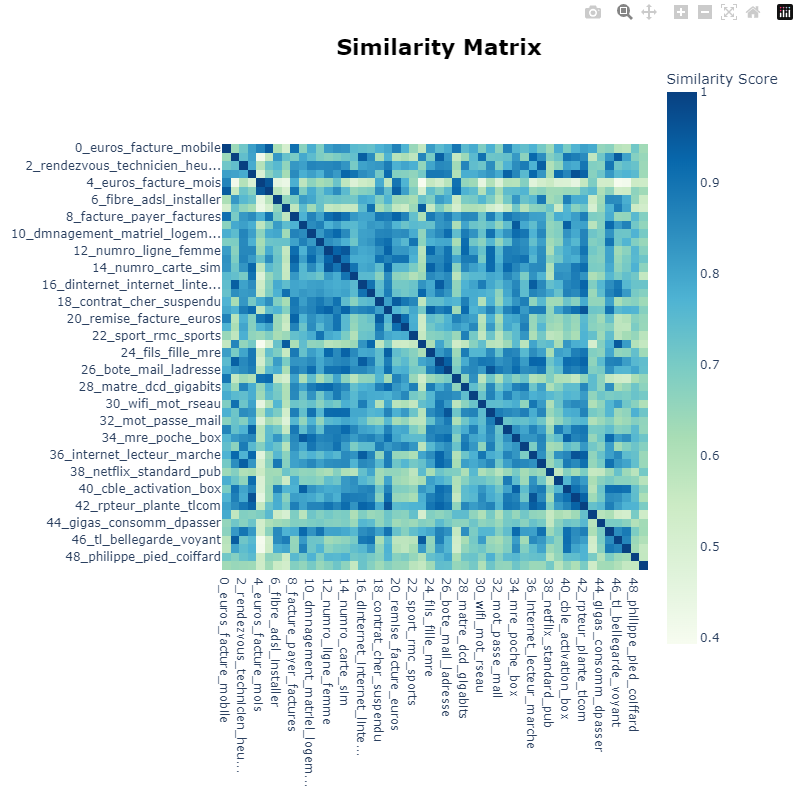
\includegraphics[width=\linewidth]{images/results/mini/hierachy_umap.png}
        \caption{Hierarchy - UMAP}
    \end{subfigure}
    \begin{subfigure}{0.45\textwidth}
        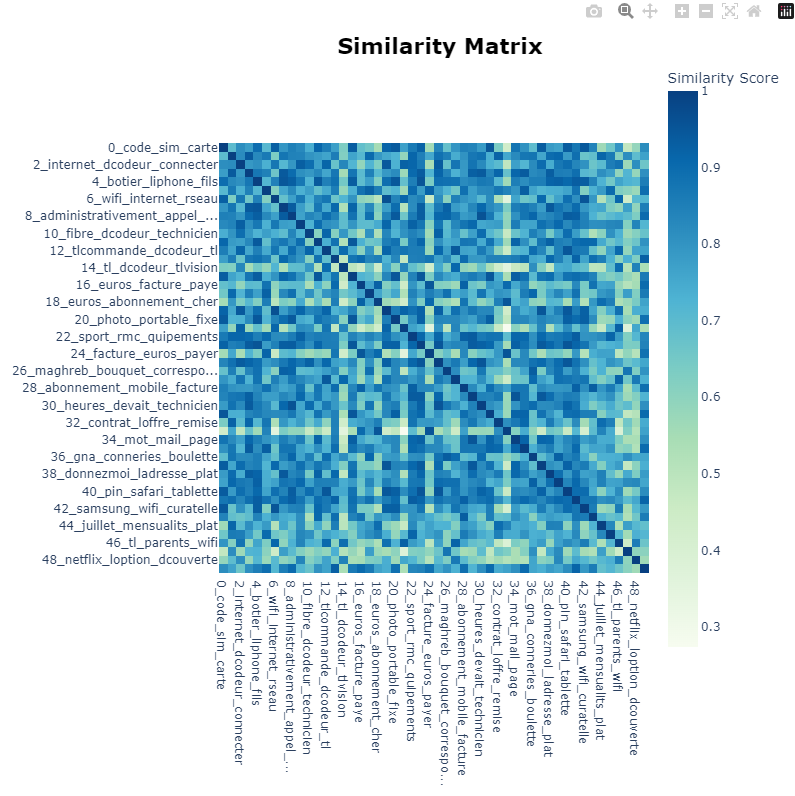
\includegraphics[width=\linewidth]{images/results/mini/hierachy_pca.png}
        \caption{Hierarchy - PCA}
    \end{subfigure}

    
    \caption{Result - miniLMv2}
    \label{fig:result_mini}
\end{figure}


\section{CamemBERT representation}

CamemBERT have a lower ability to distinguish between cluster than MiniLMv2. In the case of HDBSCAN and PCA with CamemBERT, because it is not obligated to cluster into mini clusters, it can even not separate clusters due to the close distance between data points.

% \begin{figure}[H]
%     \centering
%     \begin{subfigure}{0.43\textwidth}
%         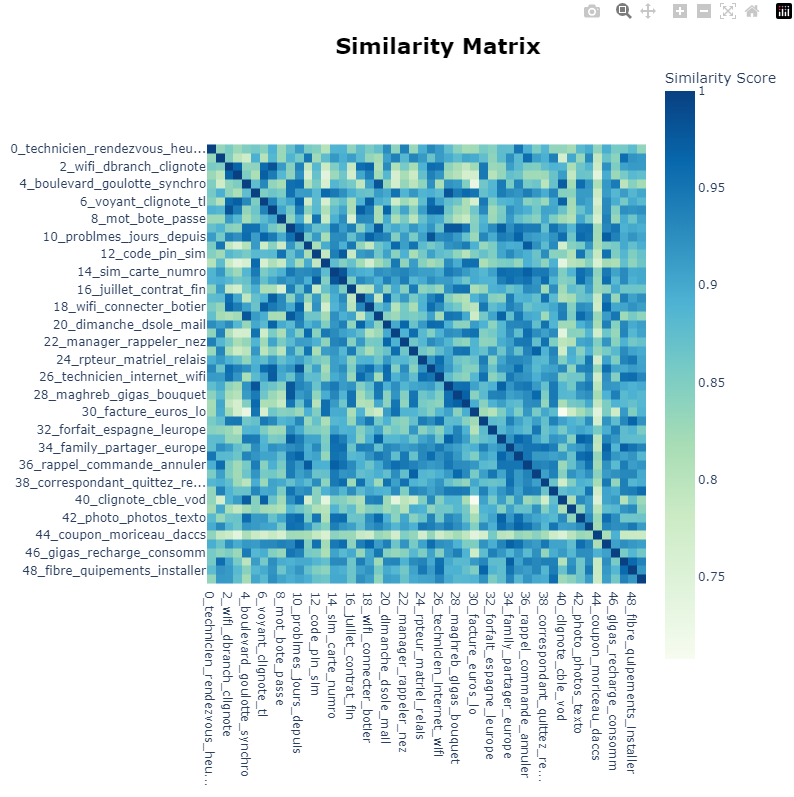
\includegraphics[width=\linewidth]{images/results/cam/kmeans_umap.png}
%         \caption{Kmeans - UMAP}
%     \end{subfigure}
%     \begin{subfigure}{0.43\textwidth}
%         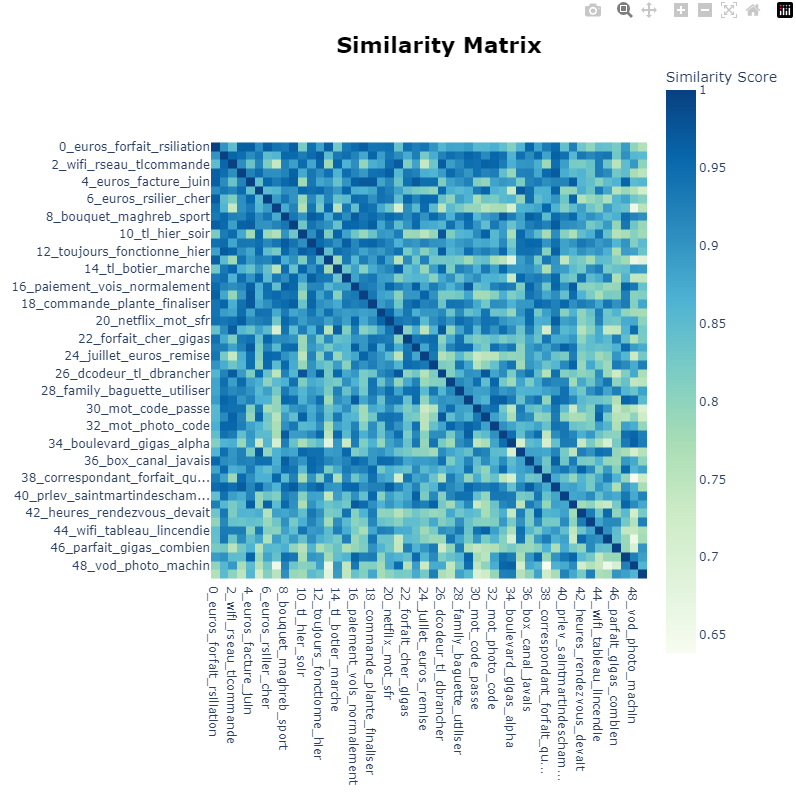
\includegraphics[width=\linewidth]{images/results/cam/kmeans_pca.png}
%         \caption{Kmeans - PCA}
%     \end{subfigure}
%     \caption{Result - CamemBERT}
%     \label{fig:result_cam_2}
% \end{figure}

\begin{figure}[H]
    \centering
        \begin{subfigure}{0.43\textwidth}
        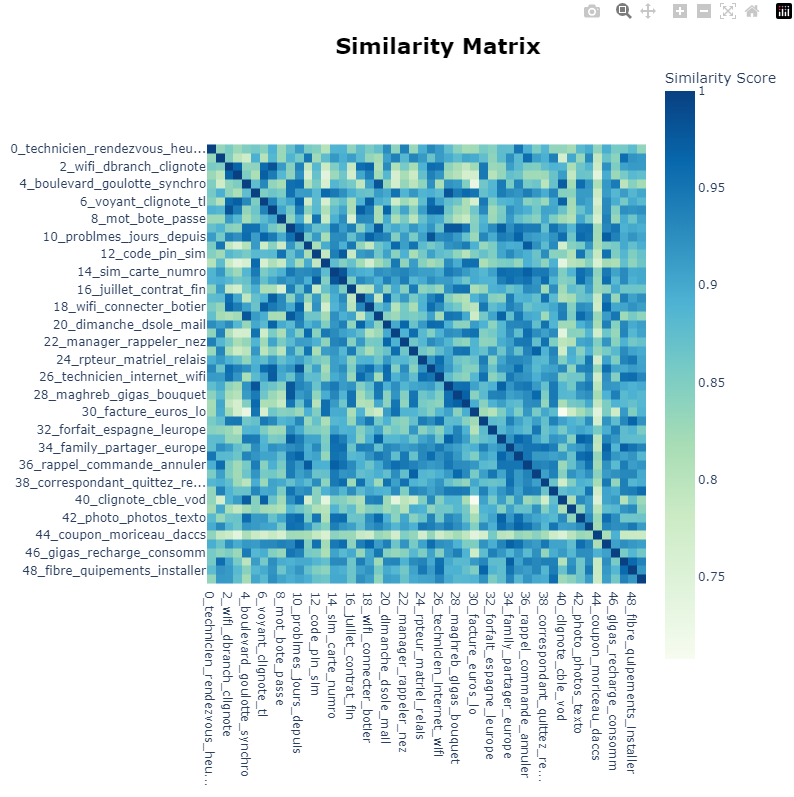
\includegraphics[width=\linewidth]{images/results/cam/kmeans_umap.png}
        \caption{Kmeans - UMAP}
    \end{subfigure}
    \begin{subfigure}{0.43\textwidth}
        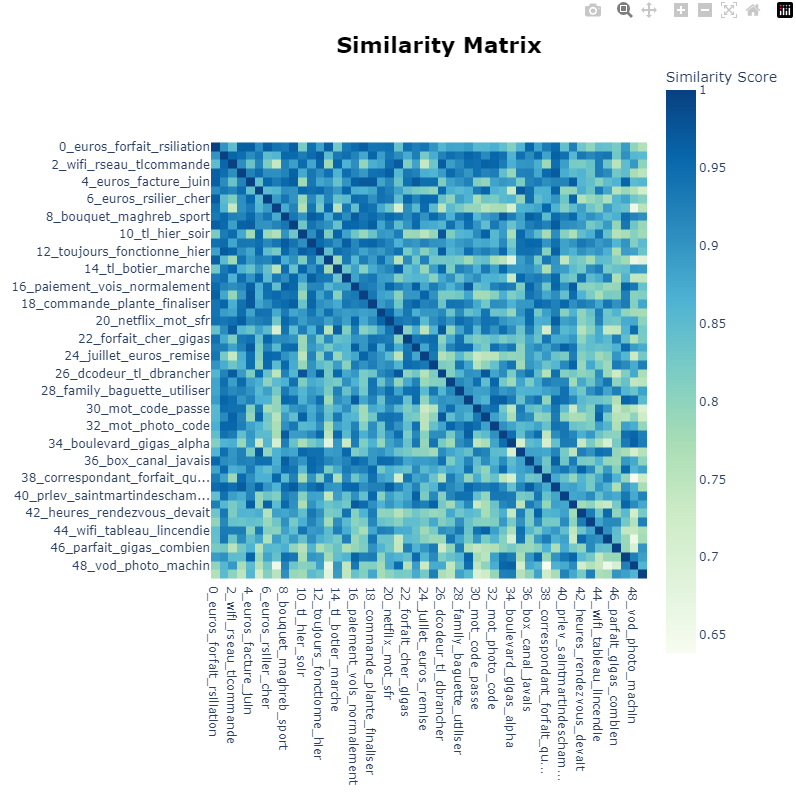
\includegraphics[width=\linewidth]{images/results/cam/kmeans_pca.png}
        \caption{Kmeans - PCA}
    \end{subfigure}
    \begin{subfigure}{0.43\textwidth}
        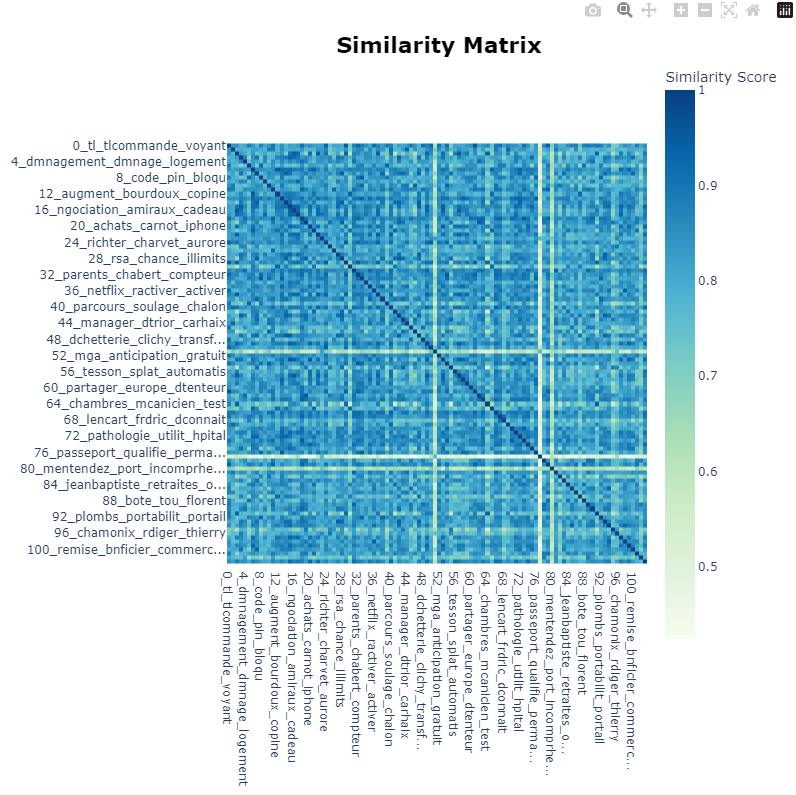
\includegraphics[width=\linewidth]{images/results/cam/hdbscan-umap.png}
        \caption{HDBSCAN - UMAP}
    \end{subfigure}
    \begin{subfigure}{0.43\textwidth}
        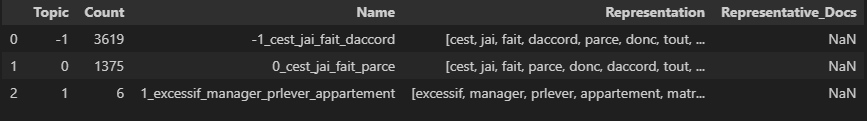
\includegraphics[width=\linewidth]{images/results/cam/hdbscan_pca.png}
        \caption{HDBSCAN - PCA}
    \end{subfigure}
    \begin{subfigure}{0.43\textwidth}
        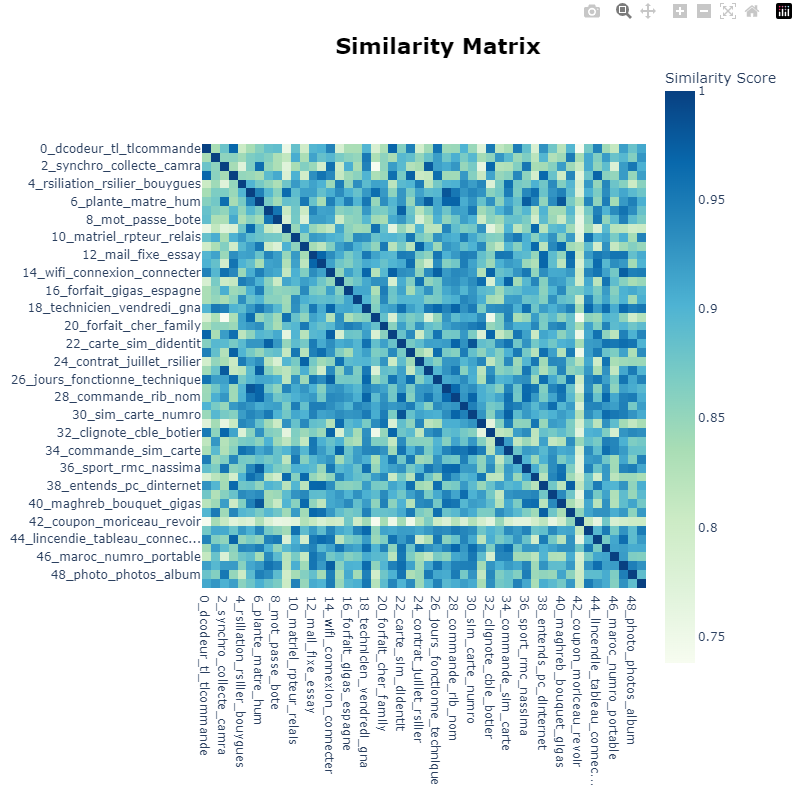
\includegraphics[width=\linewidth]{images/results/cam/hierachy_umap.png}
        \caption{Hierarchy - UMAP}
    \end{subfigure}
    \begin{subfigure}{0.43\textwidth}
        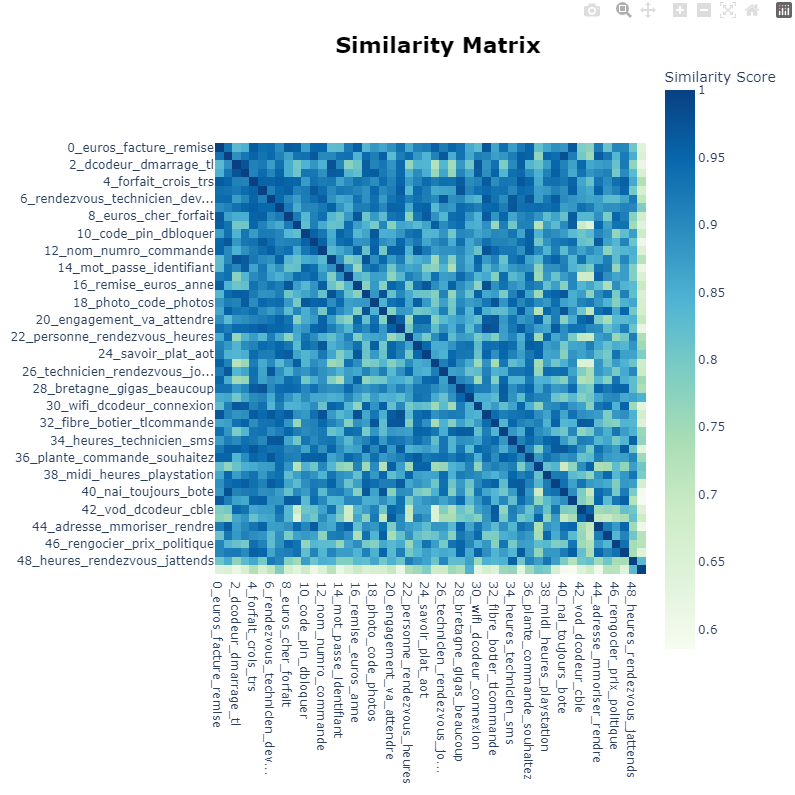
\includegraphics[width=\linewidth]{images/results/cam/hierachy_pca.png}
        \caption{Hierarchy - PCA}
    \end{subfigure}

    
    \caption{Result - CamemBERT}
    \label{fig:result_mini}
\end{figure}

\section{Hierarchy tree}

With this technique of representation, We can see which topics are closely related to each other. This is an example tree, using Hierarchy and UMAP

\begin{figure}[H]
    \centering
    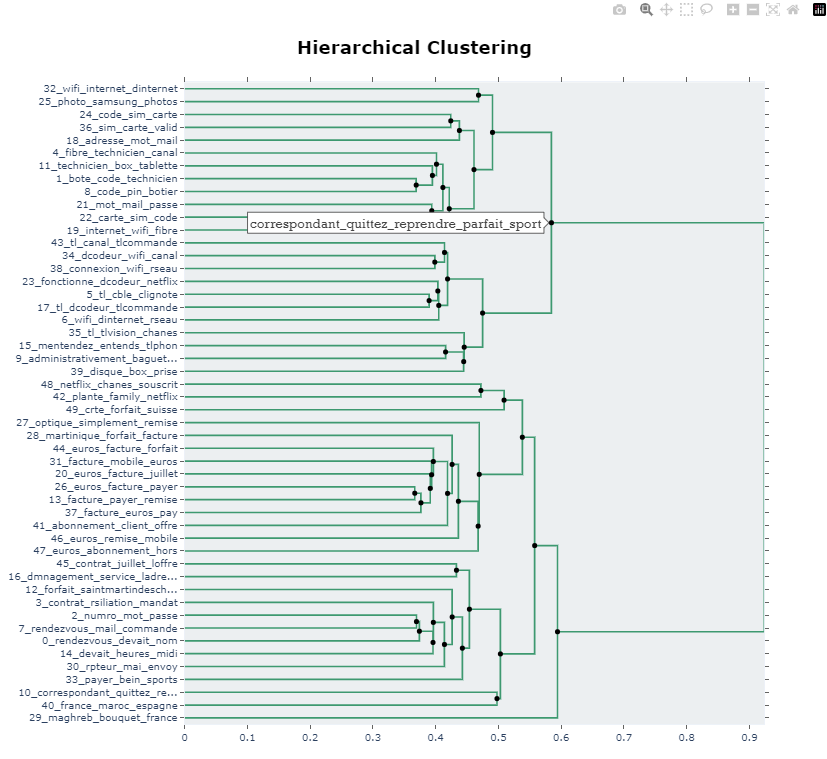
\includegraphics[width=1\textwidth]{images/results/mini/hierachy_umap_tree.png}
    \caption{Hierarchy - UMAP}
    \label{fig:hierachy_umap}
\end{figure}